\documentclass[aspectratio=169,10pt,t]{beamer}
\usepackage{issa}  % place issa.sty in the same folder
\definecolor{AccentCol}{HTML}{0D5C6F}
\renewcommand{\lecnum}{4}
\begin{document}
\titleslide{4}{Unsupervised Learning Part 1:\\Clustering \& Dimensionality Reduction}{k-Means \textbullet\ DBSCAN \textbullet\ GMM \textbullet\ Hierarchical \textbullet\ PCA \textbullet\ t-SNE \textbullet\ UMAP\\Case study: OPFOR tactical archetype discovery, N = 8,000 trajectories, JANUS wargame simulator, 12 features}

\sect{1. Motivation}
\begin{frame}{Lecture 4 --- The Core Challenge: Discover What You Don't Know to Look For}
\begin{columns}[T]
\column{0.52\textwidth}
\figc{2.3cm}{\begin{tikzpicture}
\begin{scope}\draw[ISSAgrey](0,0)rectangle(3.2,2.4);\foreach \x/\y in {0.5/1.9,0.8/1.5,0.4/1.3}{\node[pt1]at(\x,\y){};}\foreach \x/\y in {2.5/0.5,2.8/0.9,2.2/0.7}{\node[pt2]at(\x,\y){};}\foreach \x/\y in {1.6/1.9,1.9/1.6}{\node[pt3]at(\x,\y){};}\node[lab]at(1.6,-0.3){\textbf{Supervised}: every point labelled};\end{scope}
\begin{scope}[xshift=4cm]\draw[ISSAgrey](0,0)rectangle(3.2,2.4);\foreach \x/\y in {0.5/1.9,0.8/1.5,0.4/1.3,2.5/0.5,2.8/0.9,2.2/0.7,1.6/1.9,1.9/1.6,1.4/0.4}{\node[circle,fill=ISSAgrey!70,inner sep=1.2pt]at(\x,\y){};}\draw[dashed,AccentCol](0.6,1.6)circle(0.45);\draw[dashed,AccentCol](2.5,0.7)circle(0.42);\draw[dashed,AccentCol](1.75,1.75)circle(0.3);\draw[dashed,ISSAred,thick](1.4,0.4)circle(0.15);\node[lab]at(1.6,-0.3){\textbf{Unsupervised}: find the groups};\end{scope}
\end{tikzpicture}}
\begin{cbox}[ISSAnavy]{The unsupervised problem}\scriptsize \textbf{Supervised:} ``I have labelled examples --- learn to distinguish Patrol from Assault'' (needs expert annotation of every sample). \textbf{Unsupervised:} ``Here are 8,000 trajectories --- what natural groupings exist? Are there tactics we haven't thought to label?''\end{cbox}
\begin{rbox}\scriptsize\textbf{Key insight for defence:} an analyst labelling data in 2024 cannot create categories for tactics invented in 2026. Clustering discovers NOVEL patterns before analysts know to look for them.\end{rbox}
\column{0.46\textwidth}
\begin{cbox}{Learning objectives}\scriptsize\begin{te}\item Derive $k$-Means from first principles\item Apply Elbow / Silhouette for $k$ selection\item Explain DBSCAN core / border / noise logic\item Derive GMM via the EM algorithm\item Compute PCA eigenvectors from the covariance\item Distinguish t-SNE vs UMAP for visualisation\item Validate clusters with multiple metrics\end{te}\end{cbox}
\figc{2.0cm}{\begin{tikzpicture}\tikzset{F/.style={nd,text width=2.6cm,minimum height=0.75cm}}
\node[F,fill=AccentCol!15](a)at(0,0.5){\textbf{Partitional}\\$k$-Means, GMM};\node[F,fill=AccentCol!15](b)at(3.0,0.5){\textbf{Density-based}\\DBSCAN};\node[F,fill=AccentCol!15](c)at(0,-0.5){\textbf{Hierarchical}\\agglomerative (Ward)};\node[F,fill=ISSAamb!25](d)at(3.0,-0.5){\textbf{Dim.\ reduction}\\PCA, t-SNE, UMAP};\end{tikzpicture}}
\end{columns}
\end{frame}

\begin{frame}{Case Study Dataset --- OPFOR Archetype Discovery (JANUS)}
\begin{columns}[T]
\column{0.46\textwidth}
\begin{cbox}[ISSAnavy]{Source}\scriptsize JANUS wargame exercise logs (10 armies $\times$ 5-year simulation library). $N=8{,}000$ force-movement trajectories (800 per army) --- \textbf{no class labels}: we will discover them by clustering.\end{cbox}
\figc{3.3cm}{\begin{tikzpicture}[x=0.55cm,y=0.55cm]
\draw[ISSAgrey,fill=ISSAgrn!6](0,0)rectangle(9,5.5);\node[lab,anchor=north west]at(0.1,5.45){schematic trajectories on the exercise map};
\draw[ISSAblue,thick,smooth]plot coordinates{(0.5,0.6)(1.5,1.1)(2.2,0.8)(3.1,1.4)(3.6,1.0)(4.4,1.6)};\node[font=\tiny,ISSAblue]at(4.9,1.9){patrol};
\draw[ISSAred,thick,->]plot coordinates{(0.6,4.6)(2.6,4.2)(4.6,3.6)(6.6,3.0)};\node[font=\tiny,ISSAred]at(7.3,3.1){assault};
\draw[ISSAgrn,thick,->,smooth]plot coordinates{(5.0,0.5)(6.0,1.5)(7.0,2.0)(8.4,2.2)};\node[font=\tiny,ISSAgrn]at(8.1,1.7){transit};
\fill[ISSAamb](2.0,3.0)circle(0.18);\node[font=\tiny,ISSAamb!70!black]at(2.0,2.5){static};
\draw[violet,thick,->]plot coordinates{(8.6,5.2)(8.0,4.9)(8.3,4.4)(7.6,4.2)(7.9,3.7)(7.2,3.5)};\node[font=\tiny,violet]at(6.6,4.7){infiltration?};
\end{tikzpicture}}
\column{0.52\textwidth}
\figc{4.2cm}{\scriptsize\renewcommand{\arraystretch}{1.12}\begin{tabular}{llll}\toprule\multicolumn{2}{l}{\textbf{Kinematic (8)}}&\multicolumn{2}{l}{\textbf{Contextual (4)}}\\\midrule $x_1$&Avg speed (km/h) [0--120]&$x_9$&Time-of-day code [0--3]\\$x_2$&Max speed (km/h) [0--200]&$x_{10}$&Weather code [0--4]\\$x_3$&Direction-change rate (deg/min)&$x_{11}$&Mission-phase code [0--5]\\$x_4$&Formation spread (m)&$x_{12}$&Force-size category [1--4]\\$x_5$&Dwell time at waypoints (min)&&\\$x_6$&Terrain exposure index [0--1]&&\\$x_7$&Route deviation (m)&&\\$x_8$&Engagement frequency (/h)&&\\\bottomrule\end{tabular}}
\begin{wbox}\scriptsize All features are \textbf{z-score normalised}: distance-based clustering is meaningless when speed (0--200) and exposure (0--1) are on different scales.\end{wbox}
\end{columns}
\end{frame}

\sect{2. k-Means}
\begin{frame}{$k$-Means Clustering --- Minimise Within-Cluster Variance (Lloyd's Algorithm)}
\figc{2.6cm}{\begin{tikzpicture}[x=0.45cm,y=0.45cm]
\newcommand{\kpts}{\foreach \x/\y in {1/4.4,1.6/3.8,0.8/3.3,2.0/4.6,1.3/2.9}{\node[circle,fill=\pa,inner sep=1.2pt]at(\x,\y){};}\foreach \x/\y in {4.6/1.0,5.3/1.6,4.1/1.4,5.6/0.7,4.9/2.1}{\node[circle,fill=\pb,inner sep=1.2pt]at(\x,\y){};}\foreach \x/\y in {5.2/4.4,4.6/4.9,5.8/4.0,4.9/3.6}{\node[circle,fill=\pc,inner sep=1.2pt]at(\x,\y){};}}
\begin{scope}\draw[ISSAgrey](0,0)rectangle(6.6,5.6);\def\pa{ISSAgrey}\def\pb{ISSAgrey}\def\pc{ISSAgrey}\kpts\foreach \x/\y in {2.8/1.2,3.4/4.2,0.6/0.8}{\node[star,star points=5,fill=AccentCol,draw=black,inner sep=1.3pt]at(\x,\y){};}\node[lab]at(3.3,-0.6){\textbf{0} initialise $k=3$ centres};\end{scope}
\begin{scope}[xshift=4.0cm]\draw[ISSAgrey](0,0)rectangle(6.6,5.6);\def\pa{ISSAblue}\def\pb{ISSAred}\def\pc{ISSAgrn}\kpts\foreach \x/\y in {2.8/1.2,3.4/4.2,0.6/0.8}{\node[star,star points=5,fill=AccentCol,draw=black,inner sep=1.3pt]at(\x,\y){};}\node[lab]at(3.3,-0.6){\textbf{1} assign to nearest centre};\end{scope}
\begin{scope}[xshift=8.0cm]\draw[ISSAgrey](0,0)rectangle(6.6,5.6);\def\pa{ISSAblue}\def\pb{ISSAred}\def\pc{ISSAgrn}\kpts\foreach \x/\y in {1.3/3.8,4.9/1.4,5.1/4.2}{\node[star,star points=5,fill=AccentCol,draw=black,inner sep=1.3pt]at(\x,\y){};}\node[lab]at(3.3,-0.6){\textbf{2} move centre to cluster mean};\end{scope}
\begin{scope}[xshift=12.0cm]\draw[ISSAgrey](0,0)rectangle(6.6,5.6);\def\pa{ISSAblue}\def\pb{ISSAred}\def\pc{ISSAgrn}\kpts\foreach \x/\y in {1.3/3.8,4.9/1.4,5.1/4.2}{\node[star,star points=5,fill=AccentCol,draw=black,inner sep=1.3pt]at(\x,\y){};}\node[lab]at(3.3,-0.6){\textbf{3} repeat until stable};\end{scope}
\end{tikzpicture}}
\begin{columns}[T]
\column{0.50\textwidth}
\begin{fbx}{WCSS objective and the two steps}\[J=\sum_{j=1}^{k}\sum_{x_i\in C_j}\|x_i-\mu_j\|^{2}\]\[c_i=\arg\min_j\|x_i-\mu_j\|^{2},\qquad \mu_j=\frac{1}{|C_j|}\sum_{x_i\in C_j}x_i\]\end{fbx}
\column{0.48\textwidth}
\begin{tl}\item \textbf{Initialise} with $k$-means++: choose centres with probability $\propto$ squared distance from existing centres\item \textbf{Convergence:} $J$ decreases monotonically --- guaranteed to converge, NOT to the global optimum (local minima exist)\item \textbf{Remedy:} run 10+ times, keep the lowest $J$\end{tl}
\end{columns}
\end{frame}

\begin{frame}{$k$-Means --- Key Properties, Assumptions and Cost}
\begin{columns}[T]
\column{0.50\textwidth}
\figc{2.3cm}{\begin{tikzpicture}[x=0.5cm,y=0.5cm]
\begin{scope}\draw[ISSAgrey](0,0)rectangle(5,4.6);\foreach \a in {0,30,...,330}{\node[pt1]at({2.5+1.8*cos(\a)},{2.3+1.8*sin(\a)}){};}\foreach \a in {0,60,...,300}{\node[pt2]at({2.5+0.5*cos(\a)},{2.3+0.5*sin(\a)}){};}\draw[ISSAred,dashed,thick](2.5,0)--(2.5,4.6);\node[lab]at(2.5,-0.45){rings: $k$-Means cuts in half};\end{scope}
\begin{scope}[xshift=3.1cm]\draw[ISSAgrey](0,0)rectangle(5,4.6);\foreach \x/\y in {0.8/3.6,1.1/3.9,0.9/3.3,1.3/3.6,1.0/3.0,1.4/4.1,0.6/3.8}{\node[pt1]at(\x,\y){};}\foreach \x/\y in {2.8/1.0,4.2/2.2,3.4/0.6,4.6/1.0,3.0/2.4}{\node[pt2]at(\x,\y){};}\node[lab]at(2.5,-0.45){different densities};\end{scope}
\end{tikzpicture}}
\begin{cbox}[ISSAgrn]{What $k$-Means assumes}\scriptsize $\checkmark$ convex, roughly spherical clusters $\checkmark$ roughly equal size $\checkmark$ features on the same scale (z-score!) $\checkmark$ Euclidean distance meaningful.\end{cbox}
\begin{cbox}[ISSAred]{What it cannot do}\scriptsize $\times$ arbitrary shapes (rings) $\times$ very different densities $\times$ determine $k$ automatically $\times$ handle noise/outliers.\end{cbox}
\column{0.48\textwidth}
\begin{fbx}{Complexity}\[O(N\cdot k\cdot d)\ \text{per iteration}\]\end{fbx}
\begin{tl}\item Case study: $8000\times5\times12=480$K ops/iteration; 50--150 iterations $\Rightarrow\sim$50M ops, \textbf{$<0.5$ s} on a laptop\item Random initialisation may converge to a poor local minimum; $k$-means++ ($D^2$ seeding) gives \textbf{$\sim$16$\times$} better WCSS in practice\item Always use multiple restarts (\texttt{n\_init} $\ge10$)\end{tl}
\begin{ibox}\scriptsize $k$-Means is the fast first pass --- its output is also the standard initialisation for GMM later in this lecture.\end{ibox}
\end{columns}
\end{frame}

\begin{frame}{Choosing $k$ --- the Elbow Method (WCSS vs $k$)}
\begin{columns}[T]
\column{0.56\textwidth}
\figc{4.2cm}{\begin{tikzpicture}\begin{axis}[width=7.8cm,height=4.6cm,xlabel={number of clusters $k$},ylabel={WCSS},xmin=0.6,xmax=10.4,ymin=0,ymax=100000,xtick={1,...,10},ymajorgrids,scaled y ticks=false,yticklabel style={/pgf/number format/fixed}]
\addplot[AccentCol,thick,mark=*]coordinates{(1,94420)(2,52180)(3,34610)(4,24930)(5,18440)(6,15260)(7,13540)(8,12820)(9,12280)(10,11980)};
\draw[ISSAred,thick](axis cs:5,18440)circle(0.2cm);\node[font=\tiny,ISSAred,anchor=south west]at(axis cs:5.2,22000){elbow at $k{=}5$};
\node[font=\tiny,anchor=west]at(axis cs:2.15,54000){$\Delta$42,240};\node[font=\tiny,anchor=west]at(axis cs:3.15,36500){$\Delta$17,570};\node[font=\tiny,anchor=west]at(axis cs:4.15,27500){$\Delta$9,680};\node[font=\tiny,anchor=north]at(axis cs:7.5,11000){$\Delta$ = 3,180 / 1,720 / 720 / 540 / 300};
\end{axis}\end{tikzpicture}}
\column{0.42\textwidth}
\begin{tl}\item WCSS \textbf{always} falls as $k$ grows: $k=N\Rightarrow$ WCSS $=0$; $k=1\Rightarrow$ WCSS $=SS_{\text{total}}$\item Look for the ``elbow'' --- the point of diminishing returns\item Large drops from $k=2$ to 5 ($\Delta$ 42,240 $\to$ 6,490), small after\end{tl}
\begin{wbox}\scriptsize\textbf{Data pitfall:} never choose $k$ by minimising WCSS alone. The elbow can be faint or absent --- confirm with the silhouette and domain knowledge.\end{wbox}
\begin{ibox}\scriptsize Analogy: adding battalions to a front always shortens each one's sector; the question is when the extra unit stops buying much.\end{ibox}
\end{columns}
\end{frame}

\begin{frame}{Choosing $k$ --- Silhouette Analysis Confirms $k=5$}
\begin{columns}[T]
\column{0.50\textwidth}
\figc{2.4cm}{\begin{tikzpicture}[x=0.55cm,y=0.55cm]
\foreach \x/\y in {1/3,1.6/3.5,0.8/2.4,1.8/2.7,1.3/3.9}{\node[pt1]at(\x,\y){};}\foreach \x/\y in {5.6/1.2,6.2/1.8,5.2/1.7,6.4/0.9}{\node[pt2]at(\x,\y){};}
\node[pt1,inner sep=2pt,draw=black](i)at(2.4,3.1){};\draw[ISSAgrn,thick](i)--(1.0,3.0);\draw[ISSAgrn,thick](i)--(1.6,3.5);\node[font=\tiny,ISSAgrn]at(1.5,4.4){$a(i)$: own cluster};
\draw[ISSAred,thick,dashed](i)--(5.6,1.2);\draw[ISSAred,thick,dashed](i)--(5.2,1.7);\node[font=\tiny,ISSAred]at(4.5,2.9){$b(i)$: nearest other};
\end{tikzpicture}}
\begin{fbx}{Silhouette}\[s(i)=\frac{b(i)-a(i)}{\max\{a(i),b(i)\}}\in[-1,+1],\qquad S=\tfrac1N\sum_i s(i)\]\end{fbx}
\begin{tl}\item $s=+1$ well placed; $s=0$ on a boundary; $s=-1$ likely in the wrong cluster\item $S>0.70$ strong; $S>0.50$ reasonable; $S<0.25$ weak/overlapping\end{tl}
\column{0.48\textwidth}
\figc{3.2cm}{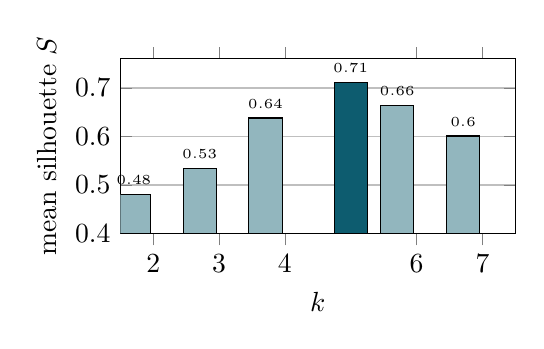
\begin{tikzpicture}\begin{axis}[ybar,width=6.6cm,height=3.8cm,symbolic x coords={2,3,4,5,6,7},xtick=data,xlabel={$k$},ylabel={mean silhouette $S$},ymin=0.4,ymax=0.76,bar width=12pt,nodes near coords,nodes near coords style={font=\fontsize{5.5}{6}\selectfont},ymajorgrids]
\addplot[fill=AccentCol!45]coordinates{(2,0.481)(3,0.534)(4,0.638)(6,0.664)(7,0.601)};\addplot[fill=AccentCol,bar shift=0pt]coordinates{(5,0.712)};
\end{axis}\end{tikzpicture}}
\begin{rbox}\scriptsize\textbf{Both methods agree: $k=5$.} Maximum silhouette $S=0.712$ --- strong evidence for five natural archetypes.\end{rbox}
\end{columns}
\end{frame}

\begin{frame}{$k=5$ Solution --- Five OPFOR Manoeuvre Archetypes Discovered}
\figc{2.8cm}{\scriptsize\renewcommand{\arraystretch}{1.18}\begin{tabular}{lrrrrrrl}\toprule\textbf{Cluster}&\textbf{Size}&\textbf{Avg spd}&\textbf{Max spd}&\textbf{Dir chg}&\textbf{Spread}&\textbf{Dwell}&\textbf{Archetype}\\\midrule C-0&1,542&18.3&42.1&3.2$^\circ$&420 m&22.4 m&PATROL (slow, spread, dwell)\\C-1&932&62.7&118.4&28.4$^\circ$&85 m&1.8 m&ASSAULT (fast, tight, no dwell)\\C-2&714&41.2&84.6&6.1$^\circ$&310 m&4.2 m&TRANSIT (medium, purposeful)\\C-3&2,184&4.8&12.3&1.2$^\circ$&380 m&61.2 m&STATIC / DEFENSIVE (long dwell)\\\rowcolor{ISSAamb!25}C-4&628&29.4&68.1&18.7$^\circ$&140 m&8.6 m&\textbf{INFILTRATION} (tight, evasive)\\\bottomrule\end{tabular}}
\begin{columns}[T]
\column{0.50\textwidth}
\figc{2.6cm}{\begin{tikzpicture}\begin{axis}[width=6.8cm,height=3.4cm,xlabel={avg speed (km/h)},ylabel={dir.\ change (deg/min)},xmin=0,xmax=70,ymin=0,ymax=32,ymajorgrids]
\addplot[only marks,mark=*,mark size=2.4pt,ISSAblue]coordinates{(18.3,3.2)};\addplot[only marks,mark=triangle*,mark size=3pt,ISSAred]coordinates{(62.7,28.4)};\addplot[only marks,mark=square*,mark size=2.2pt,ISSAgrn]coordinates{(41.2,6.1)};\addplot[only marks,mark=diamond*,mark size=3pt,ISSAamb]coordinates{(4.8,1.2)};\addplot[only marks,mark=pentagon*,mark size=3pt,violet]coordinates{(29.4,18.7)};
\node[font=\tiny,anchor=west]at(axis cs:19.5,4.5){PATROL};\node[font=\tiny,anchor=east]at(axis cs:61,28.4){ASSAULT};\node[font=\tiny,anchor=west]at(axis cs:42.5,6.1){TRANSIT};\node[font=\tiny,anchor=west]at(axis cs:6,2.4){STATIC};\node[font=\tiny,violet,anchor=west]at(axis cs:30.5,18.7){INFILTRATION};
\end{axis}\end{tikzpicture}}
\sm{Cluster centroids in two of the 12 dimensions.}
\column{0.48\textwidth}
\begin{rbox}\scriptsize\textbf{Tactical gold:} cluster C-4 (INFILTRATION) was NOT in the original analyst label schema. Moderate speed, tight formation, evasive direction changes, night-biased (time-of-day = 3) --- labelled post hoc after domain experts reviewed its members. \textbf{Unsupervised ML discovered a new enemy tactic.}\end{rbox}
\end{columns}
\end{frame}

\begin{frame}{$k=5$ Validation --- Per-Cluster Silhouette and Expert Agreement}
\begin{columns}[T]
\column{0.50\textwidth}
\subhead{Silhouette per cluster (overall mean 0.712)}
\figc{2.9cm}{\bars{1}{2.0}{1.5}{PATROL/0.741/ISSAblue,ASSAULT/0.768/ISSAred,TRANSIT/0.682/ISSAgrn,STATIC/0.801/ISSAamb,INFILTR./0.631/violet}}
\begin{tl}\item STATIC is the most distinct (0.801); TRANSIT overlaps with C-4; INFILTRATION overlaps C-1 \& C-2 (0.631)\end{tl}
\column{0.48\textwidth}
\subhead{Agreement with 200 analyst-labelled trajectories (\%)}
\figc{2.9cm}{\bars{100}{2.0}{1.5}{PATROL/91.3/ISSAblue,ASSAULT/88.7/ISSAred,TRANSIT/84.2/ISSAgrn,STATIC/94.6/ISSAamb,INFILTR./76.4/violet}}
\begin{rbox}\scriptsize Overall \textbf{87.0\%} expert--cluster alignment. INFILTRATION is lowest --- expected, since it is a \emph{new} category the analysts had no prior label for.\end{rbox}
\end{columns}
\end{frame}

\sect{3. DBSCAN}
\begin{frame}{DBSCAN --- Density-Based Clustering: Any Shape, and Outliers Flagged as Noise}
\begin{columns}[T]
\column{0.50\textwidth}
\figc{3.3cm}{\begin{tikzpicture}[x=0.7cm,y=0.7cm]
\draw[ISSAgrey](0,0)rectangle(7,4.6);
\foreach \x/\y in {1.0/2.4,1.4/2.8,1.8/2.3,1.2/1.9,1.6/1.6,2.2/2.0,2.0/2.8,2.6/2.4}{\node[circle,fill=AccentCol,inner sep=1.4pt]at(\x,\y){};}
\draw[AccentCol,dashed](1.6,2.3)circle(0.7);\node[font=\tiny,AccentCol]at(1.6,3.25){$\varepsilon$};
\node[circle,fill=ISSAamb,inner sep=1.4pt]at(3.2,2.6){};\node[font=\tiny,ISSAamb!70!black,anchor=west]at(3.3,2.6){border};
\foreach \x/\y in {4.6/1.0,5.0/1.4,5.4/1.0,5.1/0.6,5.8/1.5,4.8/1.8,5.5/2.0}{\node[circle,fill=ISSAblue,inner sep=1.4pt]at(\x,\y){};}
\foreach \x/\y in {6.4/4.0,0.5/4.2,3.8/4.1}{\node[circle,fill=ISSAred,inner sep=1.8pt]at(\x,\y){};}\node[font=\tiny,ISSAred,anchor=north]at(3.8,4.0){noise};
\node[lab,anchor=west]at(0.1,-0.35){\textcolor{AccentCol}{$\bullet$} core \ \textcolor{ISSAamb}{$\bullet$} border \ \textcolor{ISSAred}{$\bullet$} noise (cluster $=-1$)};
\end{tikzpicture}}
\begin{fbx}{Definitions}\[\text{core}(p)\iff\big|\{x:d(p,x)\le\varepsilon\}\big|\ge\text{MinPts}\]\[\text{cluster}=\text{maximal density-connected set}\]\end{fbx}
\column{0.48\textwidth}
\begin{tl}\item \textbf{Core:} $\ge$ MinPts points within its $\varepsilon$-ball\item \textbf{Border:} within $\varepsilon$ of a core point but fewer than MinPts neighbours\item \textbf{Noise:} neither --- labelled as outlier\item \textbf{Directly density-reachable:} $d(x,y)\le\varepsilon$ and $y$ is core; \textbf{density-connected:} both reachable from a common core point\item \textbf{Algorithm:} for each unvisited $p$: if core, expand the cluster; else mark as noise (may be reassigned)\item \textbf{Complexity:} $O(N\log N)$ with a spatial index\end{tl}
\begin{ibox}\scriptsize Unlike $k$-Means, DBSCAN discovers $k$ automatically and never forces an odd point into a cluster.\end{ibox}
\end{columns}
\end{frame}

\begin{frame}{DBSCAN vs $k$-Means --- and the 142 Deception Manoeuvres}
\begin{columns}[T]
\column{0.50\textwidth}
\figc{1.8cm}{\scriptsize\renewcommand{\arraystretch}{1.15}\begin{tabular}{lll}\toprule&\textbf{$k$-Means}&\textbf{DBSCAN}\\\midrule Shape&spherical / convex&\textbf{any shape}\\Noise&forced into a cluster&\textbf{labelled explicitly}\\$k$&required input&\textbf{discovered}\\\bottomrule\end{tabular}}
\subhead{Case study ($\varepsilon=0.45$, MinPts $=8$)}
\figc{2.5cm}{\bars{3500}{1.7}{1.5}{A: Patrol + Static/3214/ISSAblue,B: Assault/1847/ISSAred,C: Transit/2397/ISSAgrn,D: Infiltration/400/violet,NOISE/142/ISSAamb}}
\column{0.48\textwidth}
\begin{wbox}\scriptsize\textbf{The 142 noise points (1.78\%) = deception manoeuvres!} Zero dwell, random direction changes, night operations, unusual speed patterns --- deliberate adversary deception.\end{wbox}
\begin{cbox}[ISSAnavy]{Why this matters}\scriptsize In defence, ``noise'' is often the most interesting signal: rare or unusual behaviour. $k$-Means would have forced each of these 142 trajectories into its nearest archetype, hiding them in plain sight.\end{cbox}
\begin{ibox}\scriptsize Note: DBSCAN merged PATROL and STATIC into one dense cluster A --- density-based and centroid-based methods see different structure. Use both.\end{ibox}
\end{columns}
\end{frame}

\begin{frame}{DBSCAN --- Tuning $\varepsilon$ and MinPts with the $k$-Distance Plot}
\begin{columns}[T]
\column{0.52\textwidth}
\figc{3.5cm}{\begin{tikzpicture}\begin{axis}[width=7.2cm,height=4.2cm,xlabel={points sorted by 8th-NN distance (percentile, ascending)},ylabel={8th-NN distance},xmin=0,xmax=100,ymin=0,ymax=2,ymajorgrids]
\addplot[AccentCol,thick,mark=*,mark size=1.2pt]coordinates{(1,0.21)(10,0.32)(20,0.41)(30,0.47)(40,0.58)(50,0.72)(90,1.84)};
\draw[dashed,ISSAred](axis cs:0,0.45)--(axis cs:100,0.45);\node[font=\tiny,ISSAred,anchor=south west]at(axis cs:31,0.47){knee: $\varepsilon=0.45$};
\end{axis}\end{tikzpicture}}
\sm{Recast from the reported percentile table (99th\%ile of closeness = 0.21 \ldots\ 10th = 1.84): dense core first, isolated points last.}
\column{0.46\textwidth}
\begin{cbox}{How to choose $\varepsilon$}\scriptsize (1) For each point compute the distance to its MinPts-th nearest neighbour; (2) sort ascending; (3) plot; (4) choose $\varepsilon$ at the knee (sharp change).\end{cbox}
\subhead{MinPts: noise fraction is sensitive}
\figc{2.0cm}{\bars{350}{1.4}{2.0}{MinPts 5: 42 (0.5\%) too few/42/ISSAamb,MinPts 8: 142 (1.8\%) balanced/142/ISSAgrn,MinPts 15: 318 (4.0\%) too many/318/ISSAred}}
\begin{ibox}\scriptsize Rule of thumb MinPts $\ge d+1=13$ for $d=12$ --- but the operational noise rate (1.8\%) favoured MinPts $=8$.\end{ibox}
\end{columns}
\end{frame}

\begin{frame}{DBSCAN in Operations --- From Noise Points to a New OPFOR Doctrine Category}
\begin{columns}[T]
\column{0.50\textwidth}
\subhead{Profile of the 142 noise trajectories}
\figc{2.5cm}{\bars{100}{1.7}{1.9}{Night operations/89/ISSAnavy,Single-unit (small cell)/82/ISSAred,Near-zero dwell/100/ISSAamb}}
\sm{``Near-zero dwell at ALL waypoints'' is reported qualitatively; plotted as 100\% for illustration.}
\begin{tl}\item Avg direction change \textbf{34.2 deg/min} (vs 28.4 ASSAULT, 18.7 INFILTRATION)\item Route deviation \textbf{820 m+} from the shortest path\end{tl}
\column{0.48\textwidth}
\begin{rbox}\scriptsize\textbf{Expert conclusion:} DELIBERATE DECEPTION MANOEUVRES --- small units moving erratically to confuse pattern-of-life analysis. \textbf{Action:} a new OPFOR doctrine SOP for deceptive manoeuvres, added as explicit Category 6 in training.\end{rbox}
\begin{wbox}\scriptsize\textbf{DBSCAN limitation:} struggles with clusters of VARYING density --- common in real data (dense urban trajectories vs sparse rural). \textbf{HDBSCAN} converts DBSCAN to a hierarchy via a single-linkage tree and extracts stable clusters at multiple density scales: recommended for real intelligence data.\end{wbox}
\end{columns}
\end{frame}

\sect{4. Gaussian Mixtures}
\begin{frame}{Gaussian Mixture Models --- Each Cluster Is a Gaussian: Soft Assignment by Probability}
\begin{columns}[T]
\column{0.48\textwidth}
\figc{2.9cm}{\begin{tikzpicture}[x=0.6cm,y=0.6cm]
\draw[ISSAgrey](0,0)rectangle(8,5);
\draw[ISSAblue,fill=ISSAblue!12,rotate around={30:(2.3,3.1)}](2.3,3.1)ellipse(1.9 and 0.9);\draw[ISSAred,fill=ISSAred!12,rotate around={-25:(5.6,2.0)}](5.6,2.0)ellipse(1.6 and 0.6);\draw[ISSAgrn,fill=ISSAgrn!12](5.8,4.0)ellipse(0.8 and 0.5);
\foreach \x/\y in {1.2/2.4,2.0/3.0,2.8/3.6,3.2/3.9,1.7/2.6,2.5/3.2}{\node[circle,fill=ISSAblue,inner sep=1pt]at(\x,\y){};}\foreach \x/\y in {4.6/2.5,5.4/2.1,6.3/1.6,5.0/2.3,6.7/1.4}{\node[circle,fill=ISSAred,inner sep=1pt]at(\x,\y){};}
\node[circle,fill=violet,draw=black,inner sep=1.8pt](t)at(4.0,2.9){};\node[font=\tiny,violet,anchor=south]at(4.0,3.05){$T_{481}$: 0.62 / 0.38};
\end{tikzpicture}}
\begin{fbx}{Mixture model and responsibility}\[P(x)=\sum_{k=1}^{K}\pi_k\,\mathcal{N}(x;\mu_k,\Sigma_k),\quad\sum_k\pi_k=1\]\[r_{ik}=\frac{\pi_k\mathcal{N}(x_i;\mu_k,\Sigma_k)}{\sum_j\pi_j\mathcal{N}(x_i;\mu_j,\Sigma_j)}\in[0,1]\]\end{fbx}
\column{0.50\textwidth}
\begin{tl}\item $\pi_k$: mixture weight; $\mu_k$: mean; $\Sigma_k$: covariance (shape and orientation)\item Each point belongs \emph{partially} to ALL clusters: $\sum_kr_{ik}=1$\end{tl}
\figc{2.3cm}{\scriptsize\renewcommand{\arraystretch}{1.15}\begin{tabular}{lll}\toprule&\textbf{$k$-Means}&\textbf{GMM}\\\midrule Assignment&hard (one cluster)&\textbf{soft (probabilities)}\\Shape&spherical ($\Sigma=\sigma^2I$)&\textbf{elliptical (full $\Sigma_k$)}\\Relation&special case of GMM: $\Sigma_k=\sigma^2I$, $\sigma\to0$&\\\bottomrule\end{tabular}}
\begin{rbox}\scriptsize\textbf{Benefit:} trajectory $T_{481}$ has $r(\text{ASSAULT})=0.62$, $r(\text{INFILTRATION})=0.38$ $\Rightarrow$ alert analysts that it is \emph{ambiguous} instead of silently labelling it ASSAULT.\end{rbox}
\end{columns}
\end{frame}

\begin{frame}{GMM Case Study --- Model Selection with AIC and BIC}
\begin{columns}[T]
\column{0.52\textwidth}
\figc{3.4cm}{\begin{tikzpicture}\begin{axis}[width=7.2cm,height=4.1cm,xlabel={number of components $K$},ylabel={criterion (lower = better)},xmin=2.6,xmax=7.4,ymin=49000,ymax=52200,xtick={3,...,7},ymajorgrids,legend pos=north east,scaled y ticks=false,yticklabel style={/pgf/number format/fixed}]
\addplot[AccentCol,thick,mark=*]coordinates{(3,51240)(4,49820)(5,49432)(6,49680)(7,50010)};\addlegendentry{AIC}
\addplot[ISSAred,thick,mark=square*]coordinates{(3,51890)(4,50640)(5,50540)(6,51020)(7,51590)};\addlegendentry{BIC}
\node[font=\tiny,ISSAgrn,anchor=north]at(axis cs:5,49380){best: $K=5$};
\end{axis}\end{tikzpicture}}
\begin{fbx}{Information criteria ($p$ parameters)}\[\text{AIC}=2p-2\log L,\qquad\text{BIC}=p\log N-2\log L\]\end{fbx}
\column{0.46\textwidth}
\begin{ibox}\scriptsize BIC penalises extra parameters more heavily than AIC. Here both are minimised at $K=5$ (AIC 49,432; BIC 50,540; log-likelihood $-24{,}516$). Log-likelihood keeps rising with $K$ ($-24{,}205$ at $K=7$) --- never select on likelihood alone.\end{ibox}
\subhead{$K=5$ cluster profiles (mixture weights $\pi$)}
\figc{2.3cm}{\bars{0.3}{1.5}{1.5}{PATROL wide $\Sigma$/0.193/ISSAblue,ASSAULT tight/0.117/ISSAred,TRANSIT elongated/0.089/ISSAgrn,STATIC near-zero $\mu_v$/0.272/ISSAamb,INFILTR. diagonal/0.079/violet}}
\end{columns}
\end{frame}

\begin{frame}{The EM Algorithm --- Maximum Likelihood for GMM by Alternating E- and M-Steps}
\begin{columns}[T]
\column{0.52\textwidth}
\begin{fbx}{Goal and E-step}\[\mathcal{L}(\theta)=\sum_{i=1}^{N}\log\sum_k\pi_k\mathcal{N}(x_i;\mu_k,\Sigma_k)\]\[\textbf{E: }\ r_{ik}=\frac{\pi_k\mathcal{N}(x_i;\mu_k,\Sigma_k)}{\sum_j\pi_j\mathcal{N}(x_i;\mu_j,\Sigma_j)}\]\end{fbx}
\begin{fbx}{M-step}\[N_k=\sum_ir_{ik},\quad\pi_k=\tfrac{N_k}{N},\quad\mu_k=\tfrac1{N_k}\sum_ir_{ik}x_i\]\[\Sigma_k=\tfrac1{N_k}\sum_ir_{ik}(x_i-\mu_k)(x_i-\mu_k)^{\top}\]\end{fbx}
\sm{Initialise $\theta^{0}$ from $k$-Means (fast). $\mathcal{L}$ never decreases (EM theorem); stop when $|\Delta\mathcal{L}|<10^{-6}$.}
\column{0.46\textwidth}
\figc{2.5cm}{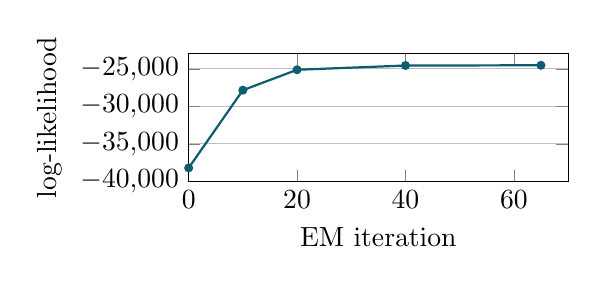
\begin{tikzpicture}\begin{axis}[width=6.4cm,height=3.2cm,xlabel={EM iteration},ylabel={log-likelihood},xmin=0,xmax=70,ymin=-40000,ymax=-23000,ymajorgrids,scaled y ticks=false,yticklabel style={/pgf/number format/fixed}]
\addplot[AccentCol,thick,mark=*,mark size=1.2pt]coordinates{(0,-38214)(10,-27840)(20,-25118)(40,-24551)(65,-24519)};\node[font=\tiny,anchor=south east]at(axis cs:65,-24400){converged at 65};
\end{axis}\end{tikzpicture}}
\begin{wbox}\scriptsize\textbf{Pitfall 1 --- local maxima:} use 10 random starts (best $-24{,}516$). \textbf{Pitfall 2 --- singularities:} a component collapsing onto one point gives $\Sigma_k\to0$, likelihood $\to\infty$; regularise $\Sigma_k\mathrel{+}=\varepsilon I$ or bound the minimum eigenvalue $\ge0.01$. \textbf{Pitfall 3 --- label switching:} cluster ``1'' differs between runs; align runs with the Hungarian algorithm.\end{wbox}
\end{columns}
\end{frame}

\sect{5. Hierarchical}
\begin{frame}{Hierarchical Clustering --- Dendrograms for Analyst Visualisation}
\begin{columns}[T]
\column{0.52\textwidth}
\figc{3.7cm}{\begin{tikzpicture}[x=1.1cm,y=1.1cm]
\draw[->](-0.3,0)--(-0.3,4.1)node[above,font=\tiny]{merge height};\foreach \h in {0.5,1,1.5,2,2.5,3,3.5}{\draw(-0.35,\h)--(-0.25,\h);}\node[font=\tiny,anchor=east]at(-0.35,1.5){1.5};\node[font=\tiny,anchor=east]at(-0.35,3.5){3.5};
\foreach \x/\l/\cl in {0/PATROL/ISSAblue,1/STATIC/ISSAamb,2/TRANSIT/ISSAgrn,3/ASSAULT/ISSAred,4/INFILTR./violet}{\node[font=\fontsize{5.5}{6}\selectfont\bfseries,\cl,rotate=30,anchor=north east]at(\x+0.1,-0.05){\l};\draw[\cl,thick](\x,0)--(\x,0.3);}
\draw[thick](3,0.3)--(3,0.83)--(4,0.83)--(4,0.3);
\draw[thick](2,0.3)--(2,1.24)--(3.5,1.24)--(3.5,0.83);
\draw[thick](0,0.3)--(0,2.11)--(1,2.11)--(1,0.3);
\draw[thick](0.5,2.11)--(0.5,3.84)--(2.75,3.84)--(2.75,1.24);
\draw[ISSAred,dashed,thick](-0.3,1.5)--(4.4,1.5);\node[font=\tiny,ISSAred,anchor=south east]at(4.4,1.52){cut at 1.5 $\to$ 5 clusters};
\end{tikzpicture}}
\sm{Schematic dendrogram from the reported merge heights (ASSAULT--INFILTRATION 0.83; final merge 3.84).}
\column{0.46\textwidth}
\begin{cbox}{Agglomerative algorithm}\scriptsize Start with $N$ singleton clusters; repeatedly merge the two \textbf{closest} clusters until one remains $\Rightarrow$ a binary merge tree (dendrogram).\end{cbox}
\figc{2.0cm}{\scriptsize\renewcommand{\arraystretch}{1.12}\begin{tabular}{ll}\toprule\textbf{Linkage}&\textbf{Effect}\\\midrule Single (min pair)&chaining; elongated clusters\\Complete (max pair)&compact, spherical\\Average (mean pair)&balanced; most common\\\rowcolor{ISSAgrn!20}\textbf{Ward} (min $\Delta$WCSS)&compact; best for defence use\\\bottomrule\end{tabular}}
\begin{tl}\item Naive $O(N^3)$; efficient $O(N^2)$: $N=8{,}000\Rightarrow\sim$64M ops $\approx$ 8 s\item Cut at the \textbf{largest vertical gap} in the dendrogram\end{tl}
\end{columns}
\end{frame}

\begin{frame}{Ward Dendrogram Case Study --- Two Different Methods, One Answer}
\begin{columns}[T]
\column{0.50\textwidth}
\subhead{Key merge heights (2,000-trajectory subsample)}
\figc{3.1cm}{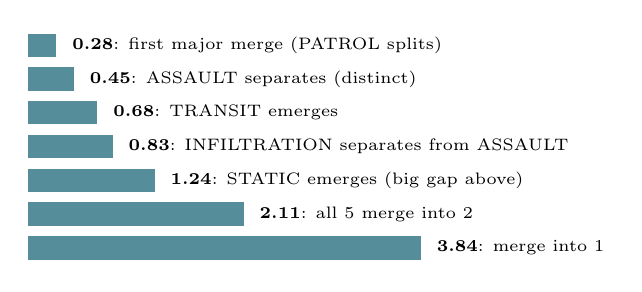
\begin{tikzpicture}[x=1cm,y=0.33cm]
\foreach \i/\h/\t in {0/0.28/first major merge (PATROL splits),1/0.45/ASSAULT separates (distinct),2/0.68/TRANSIT emerges,3/0.83/INFILTRATION separates from ASSAULT,4/1.24/STATIC emerges (big gap above),5/2.11/all 5 merge into 2,6/3.84/merge into 1}{\fill[AccentCol!70](0,-\i*1.3-0.45)rectangle(\h*1.3,-\i*1.3+0.45);\node[font=\fontsize{5.6}{6}\selectfont,anchor=west]at(\h*1.3+0.08,-\i*1.3){\textbf{\h}: \t};}
\end{tikzpicture}}
\column{0.48\textwidth}
\begin{rbox}\scriptsize\textbf{Cut at height 1.5 $\to$ 5 clusters --- matches $k$-Means.} Adjusted Rand Index between Ward ($k=5$) and $k$-Means ($k=5$): \textbf{ARI = 0.847} (1 = identical, 0 = random). Two completely different methods agree $\Rightarrow$ strong evidence for five real archetypes.\end{rbox}
\begin{cbox}[ISSAnavy]{Defence value: a visual intelligence product}\scriptsize The dendrogram shows which clusters are most alike: ASSAULT and INFILTRATION are behaviourally closest (shared speed/formation, merge height 0.83), while STATIC and PATROL are most distinct from all others. This informs COA analysis and watch-list prioritisation.\end{cbox}
\end{columns}
\end{frame}

\sect{6. PCA}
\begin{frame}{Principal Component Analysis --- Directions of Maximum Variance}
\begin{columns}[T]
\column{0.46\textwidth}
\figc{2.9cm}{\begin{tikzpicture}[x=0.7cm,y=0.7cm]
\foreach \x/\y in {-2.2/-1.1,-1.8/-0.6,-1.4/-0.9,-1.0/-0.2,-0.6/-0.5,-0.2/0.1,0.2/-0.1,0.6/0.4,1.0/0.2,1.4/0.8,1.8/0.6,2.2/1.2,-1.6/-1.2,0.9/0.7,-0.3/-0.4,1.6/1.1,-2.0/-0.8}{\node[pt1]at(\x,\y){};}
\draw[-{Stealth},AccentCol,line width=1.6pt](0,0)--(2.4,1.25)node[right,font=\scriptsize]{PC1 (most variance)};\draw[-{Stealth},ISSAred,line width=1.4pt](0,0)--(-0.45,0.85)node[above,font=\scriptsize]{PC2};
\draw[ISSAgrey,->](-2.8,0)--(2.9,0)node[right,font=\tiny]{$x_1$};\draw[ISSAgrey,->](0,-1.6)--(0,1.8)node[above,font=\tiny]{$x_2$};
\end{tikzpicture}}
\begin{ibox}\scriptsize PCA rotates the axes to line up with the data's spread, then keeps the first $k$ directions. Linear and unsupervised: it ignores clusters and labels.\end{ibox}
\column{0.52\textwidth}
\begin{fbx}{Derivation}\[\bar X=X-\text{mean}(X),\qquad C=\tfrac1N\bar X^{\top}\bar X\in\mathbb{R}^{d\times d}\]\[C=V\Lambda V^{\top},\quad\Lambda=\text{diag}(\lambda_1\ge\cdots\ge\lambda_d)\]\[\text{EVR}_j=\frac{\lambda_j}{\sum_i\lambda_i},\qquad Z=\bar XV_k\]\end{fbx}
\begin{tl}\item $C$ is symmetric PSD $\Rightarrow$ real, non-negative eigenvalues; $\lambda_j$ = variance along PC $j$\item $V_k$ = top-$k$ eigenvectors; $Z$ = PC scores ($N\times k$)\item \textbf{SVD} for numerical stability: $\bar X=USV^{\top}$, $\lambda_j=s_j^2/(N-1)$\end{tl}
\end{columns}
\end{frame}

\begin{frame}{PCA on the 12-Feature Case Study --- Four Components Explain 84.4\%}
\begin{columns}[T]
\column{0.54\textwidth}
\figc{3.6cm}{\begin{tikzpicture}\begin{axis}[width=7.4cm,height=4.3cm,xlabel={principal component},ylabel={explained variance (\%)},xmin=0.4,xmax=7.6,ymin=0,ymax=105,xtick={1,...,7},ymajorgrids,legend pos=north east]
\addplot[ybar,fill=AccentCol!65,bar width=10pt]coordinates{(1,35.1)(2,23.7)(3,13.5)(4,12.1)(5,6.0)(6,3.7)(7,2.6)};\addlegendentry{per PC}
\addplot[ISSAred,thick,mark=*]coordinates{(1,35.1)(2,58.8)(3,72.3)(4,84.4)(5,90.4)(6,94.1)(7,96.7)};\addlegendentry{cumulative}
\draw[dashed,ISSAgrey](axis cs:0.4,95)--(axis cs:7.6,95);\node[font=\tiny,anchor=south west]at(axis cs:0.5,95){95\% threshold};\node[font=\tiny,ISSAred,anchor=south east]at(axis cs:4,85){84.4\%};
\end{axis}\end{tikzpicture}}
\sm{Eigenvalues: 4.21, 2.84, 1.62, 1.45, 0.72, 0.44, 0.31, \ldots, 0.03 (PC12).}
\column{0.44\textwidth}
\begin{rbox}\scriptsize\textbf{Kaiser rule} ($\lambda>1$): keep 4 PCs (84.4\%). \textbf{95\% threshold:} 6 PCs.\end{rbox}
\begin{cbox}[ISSAred]{PC1 = ``Activity / Aggression'' axis}\scriptsize Loadings: speed 0.48, max speed 0.41, direction change 0.38.\end{cbox}
\begin{cbox}[ISSAblue]{PC2 = ``Dispersion / Caution'' axis}\scriptsize Loadings: spread 0.52, dwell time 0.44, exposure 0.31.\end{cbox}
\begin{ibox}\scriptsize Naming components from their loadings turns 12 raw features into two \emph{interpretable} tactical dimensions for briefings.\end{ibox}
\end{columns}
\end{frame}

\sect{7. t-SNE \& UMAP}
\begin{frame}{t-SNE \& UMAP --- Non-linear Dimensionality Reduction for Visualisation}
\begin{columns}[T]
\column{0.50\textwidth}
\begin{fbx}{t-SNE: match neighbourhoods}\[p_{j|i}\propto\exp\!\big(-\|x_i-x_j\|^2/2\sigma_i^2\big),\quad p_{ij}=\tfrac{p_{j|i}+p_{i|j}}{2N}\]\[q_{ij}\propto(1+\|y_i-y_j\|^2)^{-1},\qquad C=\sum_{i,j}p_{ij}\log\frac{p_{ij}}{q_{ij}}\]\end{fbx}
\begin{tl}\item PCA is linear --- cannot unfold rings or manifolds\item Student-$t$ (heavy tails) in 2-D; minimise KL by gradient descent ($\sim$1000 iterations); \textbf{perplexity} 5--50 (typ.\ 30)\item Case study (2,000 trajectories): 5 distinct clouds; INFILTRATION splits slightly from ASSAULT; STATIC isolated\end{tl}
\begin{wbox}\scriptsize\textbf{Warning:} distances BETWEEN clusters, and cluster sizes/shapes, in a t-SNE plot are NOT meaningful. Only local structure is preserved.\end{wbox}
\column{0.48\textwidth}
\figc{2.2cm}{\begin{tikzpicture}[x=0.5cm,y=0.5cm]
\draw[ISSAgrey](0,0)rectangle(9,4.4);
\foreach \cx/\cy/\cl in {1.5/3.2/ISSAblue,4.0/1.2/ISSAred,5.2/1.9/violet,3.2/3.5/ISSAgrn,8.0/2.2/ISSAamb}{\foreach \dx/\dy in {0/0,0.3/0.2,-0.3/0.15,0.15/-0.3,-0.2/-0.25,0.4/-0.1,-0.4/-0.05}{\node[circle,fill=\cl,inner sep=0.9pt]at(\cx+\dx,\cy+\dy){};}}
\node[font=\tiny]at(4.6,0.3){ASSAULT \& INFILTRATION adjacent};\node[font=\tiny,ISSAamb!70!black]at(8.0,3.1){STATIC};
\end{tikzpicture}}
\figc{2.3cm}{\scriptsize\renewcommand{\arraystretch}{1.12}\begin{tabular}{lcc}\toprule&\textbf{t-SNE}&\textbf{UMAP}\\\midrule Runtime ($N$=8,000)&38.4 s&\textbf{4.2 s} (9$\times$)\\Global structure&weak&\textbf{partly kept}\\Deterministic&no&\textbf{yes}\\Project new points&no&\textbf{yes}\\\bottomrule\end{tabular}}
\begin{rbox}\scriptsize\textbf{UMAP} ($n\_neighbors=15$, $min\_dist=0.1$): ASSAULT and INFILTRATION adjacent, STATIC maximally separated --- both correct. It can project NEW trajectories into the existing map in real time.\end{rbox}
\end{columns}
\end{frame}

\sect{8. Validation}
\begin{frame}{Cluster Validation --- How Do We KNOW the Clusters Are Real?}
\figc{3.1cm}{\scriptsize\renewcommand{\arraystretch}{1.15}\begin{tabular}{llccl}\toprule\textbf{Metric}&\textbf{Formula / method}&\textbf{Range}&\textbf{Value ($k$=5)}&\textbf{Interpretation}\\\midrule Silhouette $S$&$(b-a)/\max(a,b)$, mean&$-1$ to $+1$&0.712&strong ($>0.70$)\\Calinski--Harabasz&between / within-cluster variance&0 to $\infty$&1,842&higher = better\\Davies--Bouldin&avg max ratio within/between&0 to $\infty$&0.68&lower = better\\Dunn index&min inter / max intra distance&0 to $\infty$&0.41&higher = better\\Adjusted Rand&agreement with expert labels&$-1$ to $+1$&0.870&near-perfect alignment\\Bootstrap stability&re-cluster 100 samples, avg ARI&0 to 1&0.893&very stable\\\bottomrule\end{tabular}}
\begin{columns}[T]
\column{0.50\textwidth}
\begin{cbox}[ISSAnavy]{Gap statistic}\scriptsize $\text{Gap}(k)=E[\log\text{WCSS}_{\text{random}}(k)]-\log\text{WCSS}_{\text{data}}(k)$: compares clustering against a random baseline; choose the $k$ with maximum gap. Case study: peaks at \textbf{$k=5$}.\end{cbox}
\column{0.48\textwidth}
\begin{cbox}[ISSAnavy]{Prediction strength (Tibshirani 2005)}\scriptsize Split data, cluster both halves, measure how many co-assigned training pairs stay together in the test half; choose $k$ with PS $>0.80$. Case study: \textbf{PS = 0.887} at $k=5$.\end{cbox}
\end{columns}
\begin{rbox}\scriptsize\textbf{Verdict:} all validation measures agree --- the $k=5$ clustering is robust, stable and expert-aligned (silhouette 0.712, ARI 0.870, bootstrap stability 0.893): a high-confidence solution for operational OPFOR characterisation.\end{rbox}
\end{frame}

\begin{frame}{Algorithm Comparison --- Four Clustering Methods on 8,000 OPFOR Trajectories}
\figc{2.4cm}{\scriptsize\renewcommand{\arraystretch}{1.15}\begin{tabular}{lcccccl}\toprule\textbf{Algorithm}&\textbf{$k$ found}&\textbf{Silhouette}&\textbf{ARI}&\textbf{Noise}&\textbf{Train}&\textbf{Key strength}\\\midrule\rowcolor{ISSAgrn!20}$k$-Means ($k$=5)&5 (input)&\textbf{0.712}&\textbf{0.870}&none&0.8 s&fast, interpretable centroids\\DBSCAN ($\varepsilon$=0.45, m=8)&4 (auto)&0.684&0.821&142 (1.8\%)&2.1 s&finds noise; any shape\\GMM ($K$=5)&5 (input)&0.698&0.857&none&18.4 s&soft memberships; ellipses\\Ward hierarchical&5 (cut)&0.701&0.847&none&8.3 s&dendrogram for analysts\\\bottomrule\end{tabular}}
\figc{1.5cm}{\begin{tikzpicture}\tikzset{W/.style={ndA,text width=2.7cm,minimum height=0.9cm}}
\node[W](a)at(0,0){\textbf{1. $k$-Means}\\fast first pass};\node[W](b)at(3.4,0){\textbf{2. GMM}\\initialised from $k$-Means: probabilities};\node[W](c)at(6.8,0){\textbf{3. Hierarchical}\\visual confirmation};\node[W,fill=ISSAamb!25,draw=ISSAamb](d)at(10.2,0){\textbf{4. DBSCAN}\\noise = deception};
\draw[bigarr](a)--(b);\draw[bigarr](b)--(c);\draw[bigarr](c)--(d);\end{tikzpicture}}
\begin{columns}[T]
\column{0.33\textwidth}
\begin{cbox}[ISSAnavy]{Shapes handled}\scriptsize $k$-Means spherical; GMM elliptical; \textbf{DBSCAN any}; Ward $\approx$ spherical.\end{cbox}
\column{0.32\textwidth}
\begin{cbox}[ISSAnavy]{Finds $k$ automatically?}\scriptsize $k$-Means no; GMM only via AIC/BIC; \textbf{DBSCAN yes}; hierarchical yes (cut).\end{cbox}
\column{0.33\textwidth}
\begin{cbox}[ISSAnavy]{Scales to large $N$?}\scriptsize $k$-Means $O(Nkd)$; GMM $O(NK^2d^2)$; DBSCAN $O(N\log N)$; hierarchical \textbf{no}: $O(N^2)$ memory.\end{cbox}
\end{columns}
\end{frame}

\sect{9. Across Disciplines}
\begin{frame}{Clustering \& Dimensionality Reduction Across the Disciplines}
\subhead{Finding structure without labels is one of the oldest ideas in science}
\figc{5.0cm}{\begin{tikzpicture}
\tikzset{G/.style={nd,text width=4.75cm,align=left,minimum height=2.3cm,font=\fontsize{6.9}{8.2}\selectfont,inner sep=3pt}}
\node[G,draw=ISSAgrn,fill=ISSAgrn!7]at(-5,1.25){\textbf{\textcolor{ISSAgrn}{BIOLOGY}}\\Taxonomy and phylogenetic trees are hierarchical clusterings of species; gene-expression clustering with heat-map dendrograms (Eisen et al., 1998) found co-regulated genes.\\\textbf{Defence:} order-of-battle hierarchies inferred from observed co-movement.};
\node[G,draw=ISSAred,fill=ISSAred!6]at(0,1.25){\textbf{\textcolor{ISSAred}{ENGINEERING}}\\$k$-Means is Lloyd's algorithm, devised at Bell Labs (1957) to quantise signals for pulse-code modulation --- vector quantisation and codebooks.\\\textbf{Defence:} compressing ISR imagery over narrow UAV links; emitter codebooks in SIGINT.};
\node[G,draw=violet,fill=violet!7]at(5,1.25){\textbf{\textcolor{violet}{PSYCHOLOGY}}\\Spearman's general factor $g$ (1904) and the ``Big Five'' personality traits reduce many test scores to a few latent dimensions --- the ancestor of PCA-style reduction.\\\textbf{Defence:} summarising dozens of readiness indicators into a few axes.};
\node[G,draw=ISSAblue,fill=ISSAblue!7]at(-5,-1.25){\textbf{\textcolor{ISSAblue}{AERONAUTICS}}\\Airline flight-data monitoring clusters flight-recorder traces to find approaches unlike the rest --- before they become accidents.\\\textbf{Defence:} sortie debriefs and fleet safety; unusual profiles flagged automatically, like DBSCAN noise.};
\node[G,draw=ISSAamb,fill=ISSAyell!45]at(0,-1.25){\textbf{\textcolor{ISSAamb!80!black}{STATISTICS / EPIDEMIOLOGY}}\\John Snow's 1854 London cholera map: deaths clustered around the Broad Street pump --- spatial clustering that located a cause.\\\textbf{Defence:} incident-hotspot analysis (e.g.\ IED events) with density-based clustering.};
\node[G,draw=AccentCol,fill=AccentCol!8]at(5,-1.25){\textbf{\textcolor{AccentCol}{WARGAMING}}\\Clustering thousands of simulated runs reveals the few distinct ways a battle unfolds --- far more useful to a commander than one ``average'' outcome.\\\textbf{Use:} scenario archetypes for course-of-action comparison.};
\end{tikzpicture}}
\begin{ibox}\scriptsize\textbf{Common thread:} clusters are hypotheses, not facts. Snow still had to remove the pump handle; analysts still had to confirm the INFILTRATION archetype.\end{ibox}
\end{frame}

\sect{10. Summary}
\begin{frame}{Lecture 4 Summary --- Four Clustering Methods and Three Dimensionality-Reduction Techniques}
\figc{4.9cm}{\begin{tikzpicture}
\tikzset{K/.style={nd,text width=3.6cm,align=left,minimum height=2.1cm,font=\fontsize{6.4}{7.6}\selectfont,inner sep=3pt}}
\node[K,draw=ISSAblue,fill=ISSAblue!8]at(-4,1.2){\textbf{$k$-MEANS}\\Minimise WCSS by alternating assign + update; choose $k$ via elbow + silhouette; fast and interpretable.\\\textbf{Use:} first pass; best starting point};
\node[K,draw=ISSAamb,fill=ISSAyell!40]at(0,1.2){\textbf{DBSCAN}\\Core / border / noise via $\varepsilon$-neighbourhoods; any shape; 142 noise points = deception manoeuvres.\\\textbf{Use:} anomaly detection; no $k$ needed};
\node[K,draw=ISSAred,fill=ISSAred!7]at(4,1.2){\textbf{GMM}\\Soft memberships $r_{ik}$ fitted by EM; elliptical clusters (full $\Sigma$); AIC/BIC for $K$.\\\textbf{Use:} ambiguous boundaries};
\node[K,draw=ISSAgrn,fill=ISSAgrn!8]at(-4,-1.2){\textbf{HIERARCHICAL (WARD)}\\Dendrogram = visual intelligence product; ARI 0.847 with $k$-Means; shows cluster relationships.\\\textbf{Use:} analyst visualisation};
\node[K,draw=AccentCol,fill=AccentCol!10]at(0,-1.2){\textbf{PCA}\\Linear reduction via covariance eigenvectors; 4 PCs explain 84.4\%; PC1 activity, PC2 dispersion.\\\textbf{Use:} compression; noise removal};
\node[K,draw=violet,fill=violet!8]at(4,-1.2){\textbf{t-SNE \& UMAP}\\Non-linear 2-D maps of clusters; UMAP 9$\times$ faster and projects new points.\\\textbf{Caution:} t-SNE distances are not meaningful};
\end{tikzpicture}}
\end{frame}

\begin{frame}{Looking Ahead --- Lecture 5: Unsupervised Learning Part 2 --- Anomaly Detection}
\begin{columns}[T]
\column{0.50\textwidth}
\subhead{When ``normal'' is the label --- detecting the abnormal}
\begin{tl}\item Anomaly detection vs clustering\item Statistical methods: z-score, IQR, Mahalanobis distance; robust PCA\item \textbf{Isolation Forest:} random recursive partitioning; score = average path length; $O(N)$ training\item \textbf{One-Class SVM:} tight RBF boundary around normal; $\nu$ controls the outlier fraction\item \textbf{Autoencoders:} encode $\to$ bottleneck $\to$ decode; high reconstruction error = anomaly\item \textbf{Cyber:} SIGINT intrusion, lateral movement, command-and-control traffic\end{tl}
\begin{ibox}\scriptsize\textbf{Assignment 4:} $k$-Means derivation + DBSCAN noise analysis + one GMM EM step worked by hand.\end{ibox}
\column{0.48\textwidth}
\subhead{Preview: network intrusion, $N=500{,}000$ packets (3.6\% attacks, 41 features)}
\figc{2.7cm}{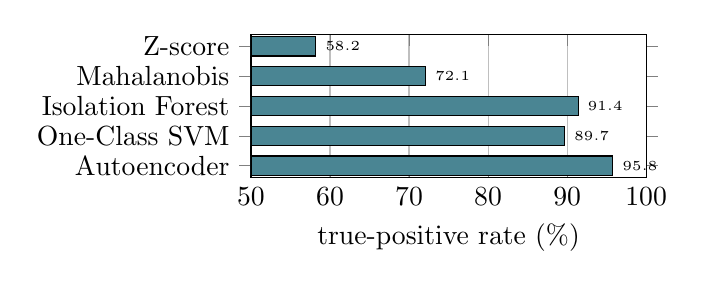
\begin{tikzpicture}\begin{axis}[xbar,width=6.6cm,height=3.4cm,symbolic y coords={Autoencoder,One-Class SVM,Isolation Forest,Mahalanobis,Z-score},ytick=data,xmin=50,xmax=100,bar width=7pt,nodes near coords,nodes near coords style={font=\fontsize{5.5}{6}\selectfont},xlabel={true-positive rate (\%)},xmajorgrids]
\addplot[fill=AccentCol!75]coordinates{(95.8,Autoencoder)(89.7,One-Class SVM)(91.4,Isolation Forest)(72.1,Mahalanobis)(58.2,Z-score)};
\end{axis}\end{tikzpicture}}
\sm{False-positive rates: 0.6\% (AE), 0.9\% (OCSVM), 1.1\% (IF), 1.8\% (Mahalanobis), 2.4\% (z-score).}
\begin{cbox}[ISSAnavy]{Insider threat module}\scriptsize 15 compromised accounts among 99.997\% normal activity: the autoencoder detects \textbf{13/15 (86.7\%)} within 48 h of the first anomalous login pattern.\end{cbox}
\end{columns}
\end{frame}
\end{document}
